\newpage
\section{Teoria uczenia maszynowego}
Informatyka z dnia na dzień, coraz śmielej wkracza we wszelkie dziedziny życia człowieka. Dzięki jej rozwojowi wiele żmudnych, uciążliwych, czy też niebezpiecznych prac wykonywanych przez człowieka może zostać zautomatyzowane. Szczególny wkład w ten gwałtowny rozwój ma konkretna dziedzina informatyki: sztuczna inteligencja. Pozwala ona na rozwiązywanie skomplikowanych zadań takich jak przetwarzanie obrazów cyfrowych, czy też analiza języka naturalnego. Ze względu na dużą ilość informacji konieczną do przeanalizowania, która zawarta jest, czy to w obrazach, czy w tekstach pisanych przez człowieka oraz ogromną różnorodność tychże danych, niezwykle problematyczne jest sformułowanie uniwersalnych algorytmów, które podjęłyby rozwiązanie problemów, jak na przykład lokalizacja obiektów w obrazach, czy ustalenie semantyki danego zdania. Z pomocą przychodzą tutaj algorytmy uczenia maszynowego należące do rodziny algorytmów sztucznej inteligencji. Pozwalają one przy pomocy uniwersalnego podejścia sformułować rozwiązanie danego problemu na podstawie historycznych danych.
\subsection{Sieci neuronowe}
Szczególnym rodzajem algorytmów uczenia maszynowego są sieci neuronowe. Zostały one stworzone na wzór neuronów obecnych w ludzkich organizmach. Składają się one z neuronów, które przetwarzają dane i przekazują do kolejnych neuronów razem tworzących warstwy. Każdy neuron posiada wagę, która jest ustalana w wyniku trenowania całej sieci przy pomocy danych dotyczących aktualnego problemu. Tak jak w przypadku ludzkiego mózgu, neurony w sieciach można komponować na wiele sposób. Do różnego rodzaju dziedzin, stosowane są różnego rodzaju architektury odpowiednio dostosowane do problemów z nimi związanych.
\subsection{Przetwarzanie języka naturalnego}
W celu przetwarzania języka naturalnego ogromną popularnością cieszą się algorytmy uczenia maszynowego, a w szczególności rekurencyjne sieci neuronowe. Ze względu na naturę języka ludzkiego, pojedyncze słowa najczęściej nie niosą ze sobą całości przekazywanych informacji -- konieczne jest wzięcie pod uwagę również kontekstu zdania, czy nawet całego tekstu. Taką możliwość dają rekurencyjne sieci neuronowe \cite{rnn}. Przy ich pomocy dane wejściowe przetwarzane są w postaci szeregu, a informacja dotycząca poprzedniego elementu jest uwzględniania przy przetwarzaniu następnego elementu. Umożliwia to również nieograniczanie długości przetwarzanych danych -- możliwe jest przetwarzanie kilku wyrazowych tekstów lub całych książek przy użyciu tej samej architektury sieci neuronowej. Schemat architektury sieci neuronowej został przedstawiony na rysunku \ref{fig:schemat-rnn}. Rekurencyjna sieć neuronowa była jednym z pierwszych takich rozwiązań oraz jednym z najpopularniejszych wykorzystywanych przy przetwarzaniu języka naturalnego. Przy jej pomocy można rozwiązać skutecznie wiele zadań, jednakże nie jest wolna od wad. Największym problemem z nią związanym jest duża niestabilność objawiająca się poprzez eksplozję lub zanikanie gradientu. Spowodowane jest to tym, iż w obliczeniach sieci rekurencyjnej za każdym razem uwzględniane są wyniki z poprzedniego przetworzenia. W przypadku chęci przetwarzania długich tekstów, mnożenie kolejnych wartości gwałtownie zwiększa lub zmniejsza wartość gradientu, co znacząco zaburza ostateczny wynik (przykładowo wartość 1,01 podniesiona do tysięcznej potęgi daje wynik ponad 10 tysięcy). W celu zaadresowania tychże problemów powstały rozszerzenia sieci rekurencyjnej. Najpopularniejsze z nich to: Long Short-term Memory \cite{lstm} oraz Gated Reccurent Unit \cite{gru}. Dzięki skomplikowaniu obliczeń oraz przekazywania danych w postaci kontekstu do kolejnych elementów szeregu, zjawisko eksplozji/zanikania gradientu nie ma tak znaczącego wpływu na ostateczne rezultaty.
\begin{figure}[!h]
  \centering
  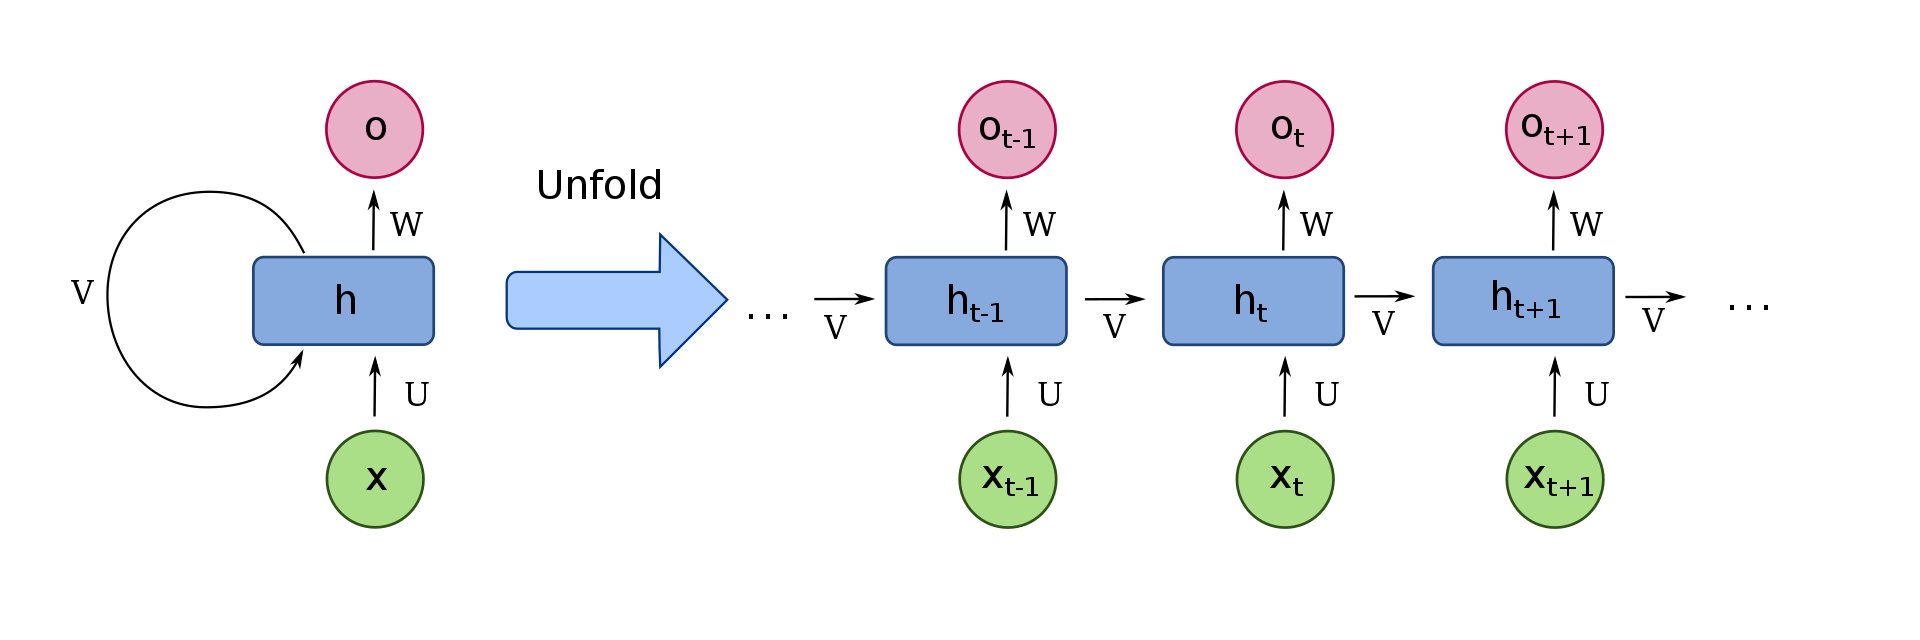
\includegraphics[width=.9\linewidth]{schemat-rnn}
  \caption{Architektura rekurencyjnej sieci neuronowej. Źródło: \cite{WikipediaEN:RNN}}
  \label{fig:schemat-rnn}
\end{figure}
\subsection{Atencja}
Atencja to kluczowy mechanizm w dziedzinie sieci neuronowych, który umożliwia modelom uczenia maszynowego skupienie się na odpowiednich częściach danych wejściowych. Jest to szczególnie przydatne w przypadku analizy sekwencji, jak również generowania podpisów do obrazków. Idea atencji opiera się na tym, że każda część danych wejściowych może mieć różne znaczenie dla wyniku. Zamiast traktować całą sekwencję jako jedną całość, atencja pozwala modelowi skupić się na istotnych fragmentach danych wejściowych w zależności od kontekstu. W praktyce atencja jest zazwyczaj implementowana jako dodatkowy moduł w sieci neuronowej. Moduł ten oblicza wagi dla poszczególnych części danych wejściowych, które określają, jak bardzo te części powinny być brane pod uwagę przy generowaniu wyniku. Wagi te są obliczane na podstawie podobieństwa między danymi wejściowymi a aktualnym stanem modelu.
\subsection{Wstępne przetwarzanie danych}
W procesie przygotowywania danych do przetwarzania przez sieci neuronowe konieczne jest dokładne ujednolicenie i przekształcenie danych w formę, która jest łatwo przyswajalna przez komputer. Dla obrazów cyfrowych, które są reprezentowane jako macierze kodów RGB, wystarcza zazwyczaj znormalizowanie wartości pikseli oraz ujednolicenie ich wymiarów w celu ułatwienia obliczeń. W przypadku wartości tekstowych, które są wartością wyjściową całej architektury, proces przetwarzania jest bardziej skomplikowany. Tekst w języku naturalnym posiada różnorodność, obejmującą zmienność długości słów, różne końcówki, a także inne nieregularności. Aby uporządkować te rozbieżności, stosuje się kilka technik:
\begin{itemize}
  \item normalizacja wielkości liter -- wszystkie litery w tekście są zamieniane na małe litery.
  \item Usunięcie wszystkich znaków niebędących słowami takich jak kropki, przecinki, emotikony.
  \item Usunięcie słów ze stop listy, czyli zbioru słów o nikłym znaczeniu dla kontekstu zdania, takich jak spójniki, przyimki lub nawet często używane słowa.
  \item W przypadku chęci osiągnięcia znaczącej generalizacji często stosowane jest również odrzucenie rzadko występujących słów w celu zmniejszenia dostępnego słownika, a co za tym idzie, zwiększenia skuteczności uczenia.
\end{itemize}
\subsection{Wizja komputerowa}
Przetwarzanie wszelkiego rodzaju obrazów cyfrowych w postaci zdjęć filmów itd. jest niezwykle problematyczne, ponieważ pojedyncze zdjęcie wykonane w jakości HD posiada prawie milion pikseli. Dodatkowo biorąc pod uwagę wiele kombinacji, w których zdjęcie może być wykonane, dane konieczne do przetworzenia oraz sformułowanie na ich podstawie algorytmów rozwiązujących dużą część problemów z nimi związanych jest praktycznie niemożliwe. Z tychże względów ogromną popularnością wśród rozwiązywania problemów związanych z wizją komputerową cieszą się algorytmy uczenia maszynowego, a w szczególności splotowe sieci neuronowe. Charakteryzują się one różnymi rodzajami warstw. Do podstawowych typów warstw należą:
\begin{itemize}
  \item warstwa splotowa -- jest to podstawowa warstwa, która składa się z zestawu filtrów splotowych wykorzystujących operację splotu. Filtry te przesuwają się po obrazie wejściowym i wykrywają w nim wzorce o różnym stopniu skomplikowania.
  \item Warstwa aktywacji -- wyniki operacji splotu są przetwarzane za pomocą funkcji aktywacji, takiej jak tangens hiperboliczny, co pozwala na generowanie tak zwanych map cech dla każdego filtra z warstwy splotowej.
  \item Warstwa grupująca -- rozmiar otrzymanych map cech wygenerowanych przez warstwę splotową jest redukowany poprzez grupowanie wartości w oknie i zastępowanie ich pojedynczą wartością reprezentującą cechy w danym obszarze. Najczęściej stosowane są dwa rodzaje operacji grupujących: max-pooling i average-pooling.
\end{itemize}
Powyższe warstwy najczęściej występują wielokrotnie w obrębie jednej sieci, co pozwala na wydobywanie wzorców z przetwarzanego obrazu na różnym poziomie kontekstu. Dalsze przetwarzanie oraz grupowanie map cech obrazu daje możliwość uwzględnienia szerszego kontekstu, jaki jest zawarty w obrazie niż jedynie w obrębie najbliższego sąsiedztwa danego piksela. Schemat podstawowej architektury splotowej sieci neuronowej służącej do klasyfikacji obrazu został przedstawiony na rysunku \ref{fig:schemat-cnn}.
\begin{figure}[!h]
  \centering
  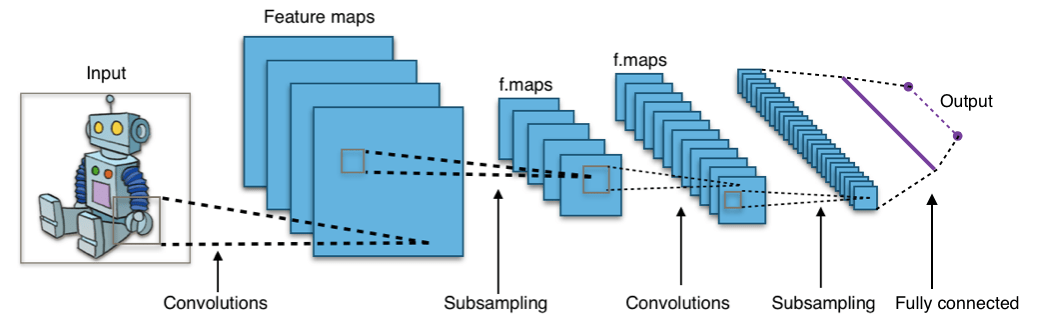
\includegraphics[width=.9\linewidth]{schemat-cnn}
  \caption{Architektura splotowej sieci neuronowej. Źródło: \cite{WikipediaEN:CNN}}
  \label{fig:schemat-cnn}
\end{figure}
